% Created by tikzDevice version 0.9 on 2016-01-11 22:38:36
% !TEX encoding = UTF-8 Unicode
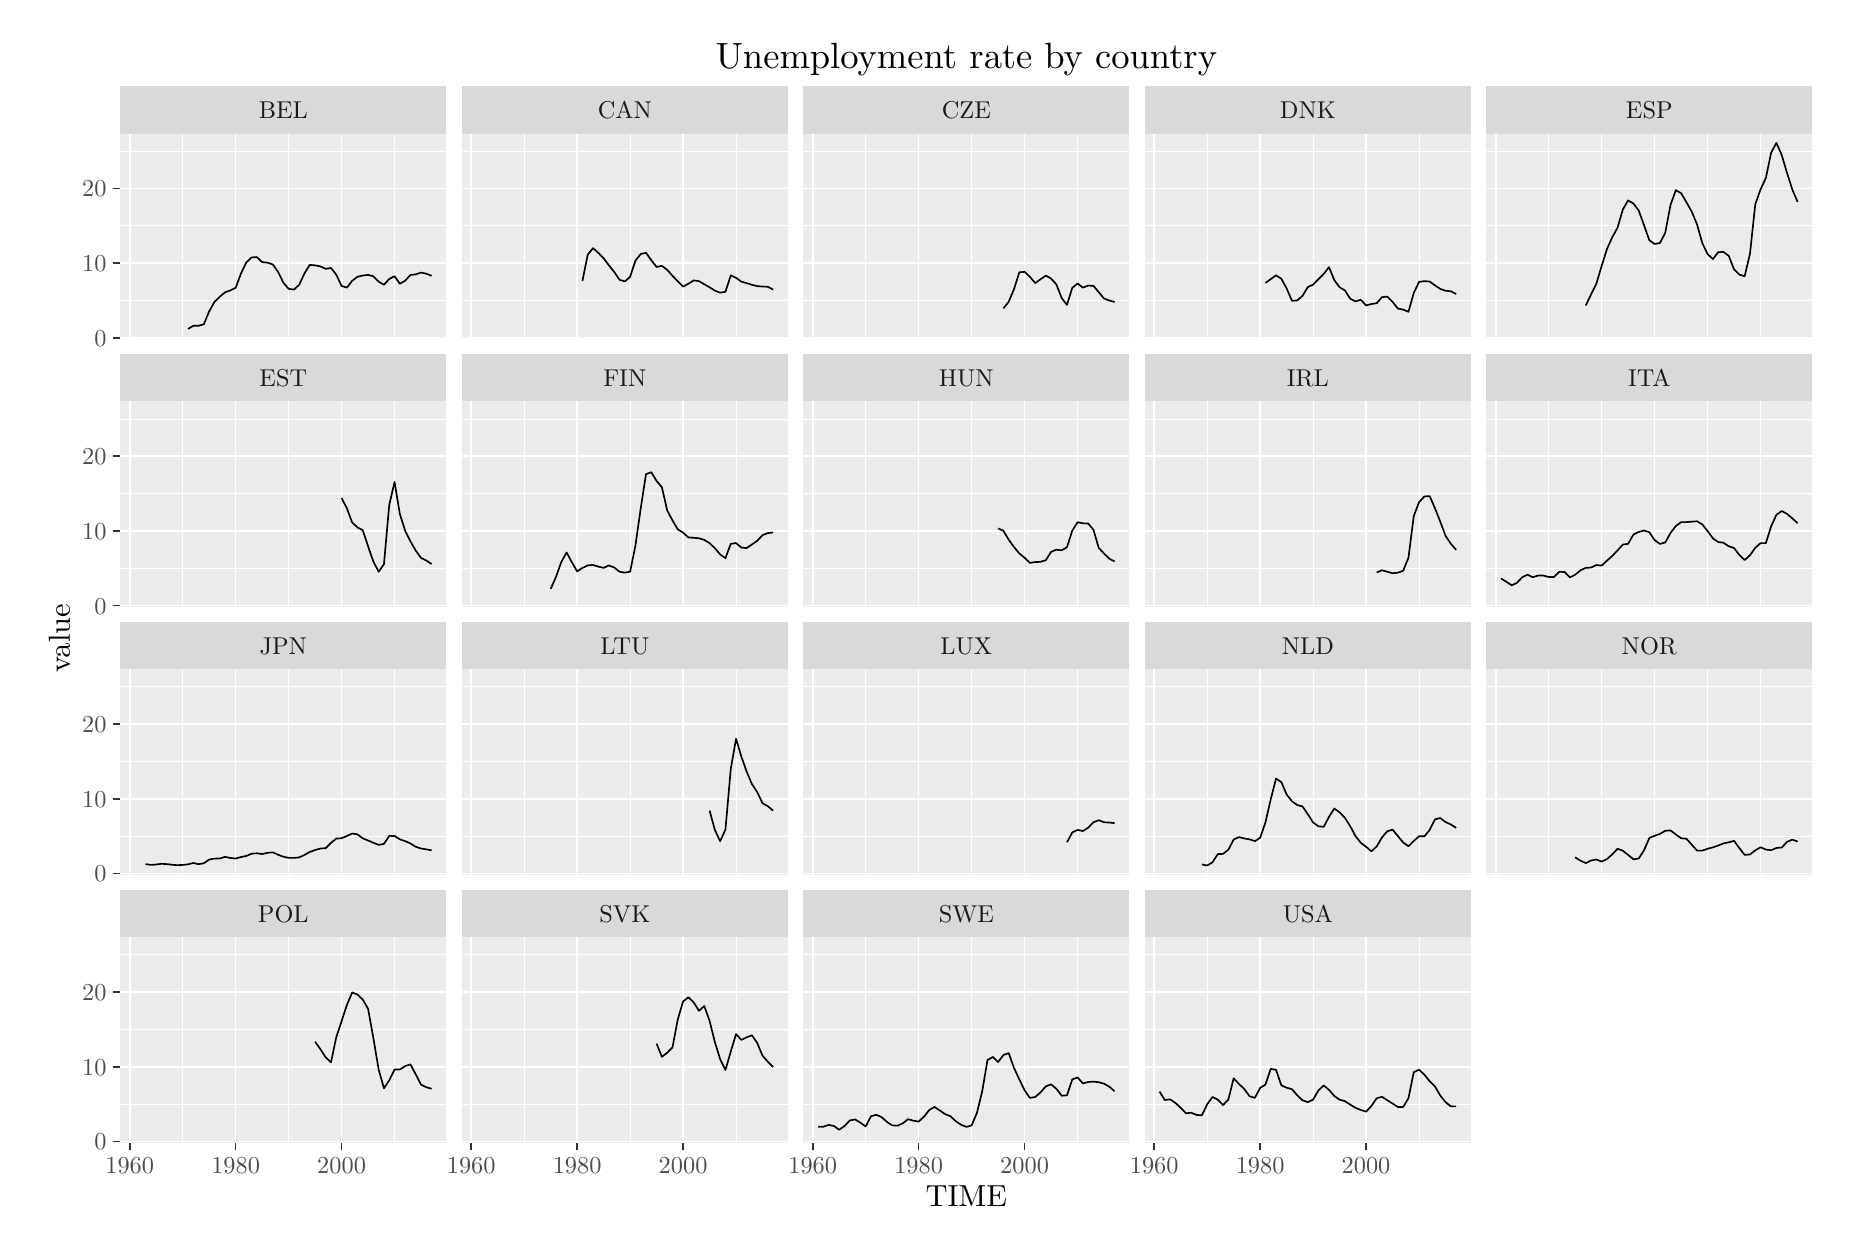
\begin{tikzpicture}[x=1pt,y=1pt]
\definecolor{fillColor}{RGB}{255,255,255}
\path[use as bounding box,fill=fillColor,fill opacity=0.00] (0,0) rectangle (650.43,433.62);
\begin{scope}
\path[clip] (  0.00,  0.00) rectangle (650.43,433.62);
\definecolor{drawColor}{RGB}{255,255,255}
\definecolor{fillColor}{RGB}{255,255,255}

\path[draw=drawColor,line width= 0.6pt,line join=round,line cap=round,fill=fillColor] (  0.00,  0.00) rectangle (650.43,433.62);
\end{scope}
\begin{scope}
\path[clip] ( 33.42,321.12) rectangle (151.33,395.37);
\definecolor{fillColor}{gray}{0.92}

\path[fill=fillColor] ( 33.42,321.12) rectangle (151.33,395.37);
\definecolor{drawColor}{RGB}{255,255,255}

\path[draw=drawColor,line width= 0.3pt,line join=round] ( 33.42,335.07) --
	(151.33,335.07);

\path[draw=drawColor,line width= 0.3pt,line join=round] ( 33.42,362.06) --
	(151.33,362.06);

\path[draw=drawColor,line width= 0.3pt,line join=round] ( 33.42,389.04) --
	(151.33,389.04);

\path[draw=drawColor,line width= 0.3pt,line join=round] ( 56.01,321.12) --
	( 56.01,395.37);

\path[draw=drawColor,line width= 0.3pt,line join=round] ( 94.29,321.12) --
	( 94.29,395.37);

\path[draw=drawColor,line width= 0.3pt,line join=round] (132.57,321.12) --
	(132.57,395.37);

\path[draw=drawColor,line width= 0.6pt,line join=round] ( 33.42,321.58) --
	(151.33,321.58);

\path[draw=drawColor,line width= 0.6pt,line join=round] ( 33.42,348.56) --
	(151.33,348.56);

\path[draw=drawColor,line width= 0.6pt,line join=round] ( 33.42,375.55) --
	(151.33,375.55);

\path[draw=drawColor,line width= 0.6pt,line join=round] ( 36.87,321.12) --
	( 36.87,395.37);

\path[draw=drawColor,line width= 0.6pt,line join=round] ( 75.15,321.12) --
	( 75.15,395.37);

\path[draw=drawColor,line width= 0.6pt,line join=round] (113.43,321.12) --
	(113.43,395.37);
\definecolor{drawColor}{RGB}{0,0,0}

\path[draw=drawColor,line width= 0.6pt,line join=round] ( 57.92,324.76) --
	( 59.84,325.88) --
	( 61.75,325.90) --
	( 63.66,326.44) --
	( 65.58,331.10) --
	( 67.49,334.50) --
	( 69.41,336.40) --
	( 71.32,337.99) --
	( 73.23,338.68) --
	( 75.15,339.63) --
	( 77.06,344.74) --
	( 78.98,348.76) --
	( 80.89,350.59) --
	( 82.80,350.72) --
	( 84.72,348.88) --
	( 86.63,348.72) --
	( 88.55,348.07) --
	( 90.46,345.40) --
	( 92.37,341.52) --
	( 94.29,339.25) --
	( 96.20,338.96) --
	( 98.12,340.72) --
	(100.03,344.86) --
	(101.94,347.91) --
	(103.86,347.73) --
	(105.77,347.35) --
	(107.69,346.47) --
	(109.60,346.79) --
	(111.51,344.36) --
	(113.43,340.29) --
	(115.34,339.69) --
	(117.26,342.13) --
	(119.17,343.60) --
	(121.08,344.05) --
	(123.00,344.29) --
	(124.91,343.78) --
	(126.83,341.82) --
	(128.74,340.72) --
	(130.65,342.81) --
	(132.57,343.82) --
	(134.48,341.08) --
	(136.40,342.18) --
	(138.31,344.25) --
	(140.22,344.47) --
	(142.14,345.12) --
	(144.05,344.71) --
	(145.97,343.96);
\end{scope}
\begin{scope}
\path[clip] (156.83,321.12) rectangle (274.73,395.37);
\definecolor{fillColor}{gray}{0.92}

\path[fill=fillColor] (156.83,321.12) rectangle (274.73,395.37);
\definecolor{drawColor}{RGB}{255,255,255}

\path[draw=drawColor,line width= 0.3pt,line join=round] (156.83,335.07) --
	(274.73,335.07);

\path[draw=drawColor,line width= 0.3pt,line join=round] (156.83,362.06) --
	(274.73,362.06);

\path[draw=drawColor,line width= 0.3pt,line join=round] (156.83,389.04) --
	(274.73,389.04);

\path[draw=drawColor,line width= 0.3pt,line join=round] (179.41,321.12) --
	(179.41,395.37);

\path[draw=drawColor,line width= 0.3pt,line join=round] (217.69,321.12) --
	(217.69,395.37);

\path[draw=drawColor,line width= 0.3pt,line join=round] (255.97,321.12) --
	(255.97,395.37);

\path[draw=drawColor,line width= 0.6pt,line join=round] (156.83,321.58) --
	(274.73,321.58);

\path[draw=drawColor,line width= 0.6pt,line join=round] (156.83,348.56) --
	(274.73,348.56);

\path[draw=drawColor,line width= 0.6pt,line join=round] (156.83,375.55) --
	(274.73,375.55);

\path[draw=drawColor,line width= 0.6pt,line join=round] (160.27,321.12) --
	(160.27,395.37);

\path[draw=drawColor,line width= 0.6pt,line join=round] (198.55,321.12) --
	(198.55,395.37);

\path[draw=drawColor,line width= 0.6pt,line join=round] (236.83,321.12) --
	(236.83,395.37);
\definecolor{drawColor}{RGB}{0,0,0}

\path[draw=drawColor,line width= 0.6pt,line join=round] (200.46,342.13) --
	(202.38,351.60) --
	(204.29,353.95) --
	(206.21,352.23) --
	(208.12,350.28) --
	(210.03,347.73) --
	(211.95,345.34) --
	(213.86,342.53) --
	(215.78,341.91) --
	(217.69,343.58) --
	(219.60,349.41) --
	(221.52,351.85) --
	(223.43,352.25) --
	(225.35,349.59) --
	(227.26,347.14) --
	(229.17,347.55) --
	(231.09,346.11) --
	(233.00,343.93) --
	(234.92,341.98) --
	(236.83,340.03) --
	(238.74,341.08) --
	(240.66,342.28) --
	(242.57,342.03) --
	(244.49,340.89) --
	(246.40,339.80) --
	(248.31,338.60) --
	(250.23,337.86) --
	(252.14,338.17) --
	(254.06,344.10) --
	(255.97,343.23) --
	(257.88,341.84) --
	(259.80,341.31) --
	(261.71,340.71) --
	(263.63,340.23) --
	(265.54,340.07) --
	(267.45,340.00) --
	(269.37,338.97);
\end{scope}
\begin{scope}
\path[clip] (280.23,321.12) rectangle (398.13,395.37);
\definecolor{fillColor}{gray}{0.92}

\path[fill=fillColor] (280.23,321.12) rectangle (398.13,395.37);
\definecolor{drawColor}{RGB}{255,255,255}

\path[draw=drawColor,line width= 0.3pt,line join=round] (280.23,335.07) --
	(398.13,335.07);

\path[draw=drawColor,line width= 0.3pt,line join=round] (280.23,362.06) --
	(398.13,362.06);

\path[draw=drawColor,line width= 0.3pt,line join=round] (280.23,389.04) --
	(398.13,389.04);

\path[draw=drawColor,line width= 0.3pt,line join=round] (302.81,321.12) --
	(302.81,395.37);

\path[draw=drawColor,line width= 0.3pt,line join=round] (341.09,321.12) --
	(341.09,395.37);

\path[draw=drawColor,line width= 0.3pt,line join=round] (379.37,321.12) --
	(379.37,395.37);

\path[draw=drawColor,line width= 0.6pt,line join=round] (280.23,321.58) --
	(398.13,321.58);

\path[draw=drawColor,line width= 0.6pt,line join=round] (280.23,348.56) --
	(398.13,348.56);

\path[draw=drawColor,line width= 0.6pt,line join=round] (280.23,375.55) --
	(398.13,375.55);

\path[draw=drawColor,line width= 0.6pt,line join=round] (283.67,321.12) --
	(283.67,395.37);

\path[draw=drawColor,line width= 0.6pt,line join=round] (321.95,321.12) --
	(321.95,395.37);

\path[draw=drawColor,line width= 0.6pt,line join=round] (360.23,321.12) --
	(360.23,395.37);
\definecolor{drawColor}{RGB}{0,0,0}

\path[draw=drawColor,line width= 0.6pt,line join=round] (352.57,332.17) --
	(354.49,334.58) --
	(356.40,339.11) --
	(358.32,345.22) --
	(360.23,345.38) --
	(362.14,343.61) --
	(364.06,341.31) --
	(365.97,342.68) --
	(367.89,344.03) --
	(369.80,342.96) --
	(371.71,340.85) --
	(373.63,335.93) --
	(375.54,333.43) --
	(377.46,339.59) --
	(379.37,341.21) --
	(381.28,339.68) --
	(383.20,340.41) --
	(385.11,340.33) --
	(387.03,338.05) --
	(388.94,335.74) --
	(390.85,335.02) --
	(392.77,334.50);
\end{scope}
\begin{scope}
\path[clip] (403.63,321.12) rectangle (521.53,395.37);
\definecolor{fillColor}{gray}{0.92}

\path[fill=fillColor] (403.63,321.12) rectangle (521.53,395.37);
\definecolor{drawColor}{RGB}{255,255,255}

\path[draw=drawColor,line width= 0.3pt,line join=round] (403.63,335.07) --
	(521.53,335.07);

\path[draw=drawColor,line width= 0.3pt,line join=round] (403.63,362.06) --
	(521.53,362.06);

\path[draw=drawColor,line width= 0.3pt,line join=round] (403.63,389.04) --
	(521.53,389.04);

\path[draw=drawColor,line width= 0.3pt,line join=round] (426.21,321.12) --
	(426.21,395.37);

\path[draw=drawColor,line width= 0.3pt,line join=round] (464.49,321.12) --
	(464.49,395.37);

\path[draw=drawColor,line width= 0.3pt,line join=round] (502.77,321.12) --
	(502.77,395.37);

\path[draw=drawColor,line width= 0.6pt,line join=round] (403.63,321.58) --
	(521.53,321.58);

\path[draw=drawColor,line width= 0.6pt,line join=round] (403.63,348.56) --
	(521.53,348.56);

\path[draw=drawColor,line width= 0.6pt,line join=round] (403.63,375.55) --
	(521.53,375.55);

\path[draw=drawColor,line width= 0.6pt,line join=round] (407.07,321.12) --
	(407.07,395.37);

\path[draw=drawColor,line width= 0.6pt,line join=round] (445.35,321.12) --
	(445.35,395.37);

\path[draw=drawColor,line width= 0.6pt,line join=round] (483.63,321.12) --
	(483.63,395.37);
\definecolor{drawColor}{RGB}{0,0,0}

\path[draw=drawColor,line width= 0.6pt,line join=round] (447.27,341.37) --
	(449.18,342.77) --
	(451.09,344.13) --
	(453.01,342.88) --
	(454.92,339.41) --
	(456.84,334.93) --
	(458.75,335.06) --
	(460.66,336.70) --
	(462.58,339.90) --
	(464.49,340.77) --
	(466.41,342.73) --
	(468.32,344.62) --
	(470.23,347.10) --
	(472.15,342.37) --
	(474.06,339.82) --
	(475.98,338.66) --
	(477.89,335.69) --
	(479.80,334.71) --
	(481.72,335.31) --
	(483.63,333.23) --
	(485.55,333.76) --
	(487.46,334.05) --
	(489.37,336.24) --
	(491.29,336.44) --
	(493.20,334.54) --
	(495.12,332.11) --
	(497.03,331.74) --
	(498.94,330.96) --
	(500.86,337.76) --
	(502.77,341.76) --
	(504.69,342.01) --
	(506.60,341.89) --
	(508.51,340.49) --
	(510.43,339.23) --
	(512.34,338.55) --
	(514.26,338.38) --
	(516.17,337.37);
\end{scope}
\begin{scope}
\path[clip] (527.03,321.12) rectangle (644.93,395.37);
\definecolor{fillColor}{gray}{0.92}

\path[fill=fillColor] (527.03,321.12) rectangle (644.93,395.37);
\definecolor{drawColor}{RGB}{255,255,255}

\path[draw=drawColor,line width= 0.3pt,line join=round] (527.03,335.07) --
	(644.93,335.07);

\path[draw=drawColor,line width= 0.3pt,line join=round] (527.03,362.06) --
	(644.93,362.06);

\path[draw=drawColor,line width= 0.3pt,line join=round] (527.03,389.04) --
	(644.93,389.04);

\path[draw=drawColor,line width= 0.3pt,line join=round] (549.61,321.12) --
	(549.61,395.37);

\path[draw=drawColor,line width= 0.3pt,line join=round] (587.89,321.12) --
	(587.89,395.37);

\path[draw=drawColor,line width= 0.3pt,line join=round] (626.17,321.12) --
	(626.17,395.37);

\path[draw=drawColor,line width= 0.6pt,line join=round] (527.03,321.58) --
	(644.93,321.58);

\path[draw=drawColor,line width= 0.6pt,line join=round] (527.03,348.56) --
	(644.93,348.56);

\path[draw=drawColor,line width= 0.6pt,line join=round] (527.03,375.55) --
	(644.93,375.55);

\path[draw=drawColor,line width= 0.6pt,line join=round] (530.47,321.12) --
	(530.47,395.37);

\path[draw=drawColor,line width= 0.6pt,line join=round] (568.75,321.12) --
	(568.75,395.37);

\path[draw=drawColor,line width= 0.6pt,line join=round] (607.03,321.12) --
	(607.03,395.37);
\definecolor{drawColor}{RGB}{0,0,0}

\path[draw=drawColor,line width= 0.6pt,line join=round] (563.01,333.24) --
	(564.93,337.22) --
	(566.84,341.10) --
	(568.75,347.51) --
	(570.67,353.61) --
	(572.58,357.87) --
	(574.50,361.37) --
	(576.41,367.91) --
	(578.32,371.20) --
	(580.24,370.06) --
	(582.15,367.53) --
	(584.07,362.22) --
	(585.98,356.80) --
	(587.89,355.46) --
	(589.81,355.80) --
	(591.72,359.46) --
	(593.64,369.57) --
	(595.55,374.90) --
	(597.46,373.81) --
	(599.38,370.56) --
	(601.29,367.16) --
	(603.21,362.53) --
	(605.12,355.77) --
	(607.03,351.79) --
	(608.95,349.99) --
	(610.86,352.48) --
	(612.78,352.57) --
	(614.69,351.16) --
	(616.60,346.26) --
	(618.52,344.39) --
	(620.43,343.79) --
	(622.35,351.95) --
	(624.26,369.77) --
	(626.17,375.17) --
	(628.09,379.30) --
	(630.00,388.47) --
	(631.91,391.99) --
	(633.83,387.53) --
	(635.74,381.11) --
	(637.66,375.08) --
	(639.57,370.64);
\end{scope}
\begin{scope}
\path[clip] ( 33.42,224.31) rectangle (151.33,298.56);
\definecolor{fillColor}{gray}{0.92}

\path[fill=fillColor] ( 33.42,224.31) rectangle (151.33,298.56);
\definecolor{drawColor}{RGB}{255,255,255}

\path[draw=drawColor,line width= 0.3pt,line join=round] ( 33.42,238.26) --
	(151.33,238.26);

\path[draw=drawColor,line width= 0.3pt,line join=round] ( 33.42,265.25) --
	(151.33,265.25);

\path[draw=drawColor,line width= 0.3pt,line join=round] ( 33.42,292.23) --
	(151.33,292.23);

\path[draw=drawColor,line width= 0.3pt,line join=round] ( 56.01,224.31) --
	( 56.01,298.56);

\path[draw=drawColor,line width= 0.3pt,line join=round] ( 94.29,224.31) --
	( 94.29,298.56);

\path[draw=drawColor,line width= 0.3pt,line join=round] (132.57,224.31) --
	(132.57,298.56);

\path[draw=drawColor,line width= 0.6pt,line join=round] ( 33.42,224.77) --
	(151.33,224.77);

\path[draw=drawColor,line width= 0.6pt,line join=round] ( 33.42,251.75) --
	(151.33,251.75);

\path[draw=drawColor,line width= 0.6pt,line join=round] ( 33.42,278.74) --
	(151.33,278.74);

\path[draw=drawColor,line width= 0.6pt,line join=round] ( 36.87,224.31) --
	( 36.87,298.56);

\path[draw=drawColor,line width= 0.6pt,line join=round] ( 75.15,224.31) --
	( 75.15,298.56);

\path[draw=drawColor,line width= 0.6pt,line join=round] (113.43,224.31) --
	(113.43,298.56);
\definecolor{drawColor}{RGB}{0,0,0}

\path[draw=drawColor,line width= 0.6pt,line join=round] (113.43,263.69) --
	(115.34,259.94) --
	(117.26,254.82) --
	(119.17,253.02) --
	(121.08,252.03) --
	(123.00,246.21) --
	(124.91,240.70) --
	(126.83,237.02) --
	(128.74,239.76) --
	(130.65,261.13) --
	(132.57,269.48) --
	(134.48,257.89) --
	(136.40,251.85) --
	(138.31,247.97) --
	(140.22,244.69) --
	(142.14,242.02) --
	(144.05,241.08) --
	(145.97,239.81);
\end{scope}
\begin{scope}
\path[clip] (156.83,224.31) rectangle (274.73,298.56);
\definecolor{fillColor}{gray}{0.92}

\path[fill=fillColor] (156.83,224.31) rectangle (274.73,298.56);
\definecolor{drawColor}{RGB}{255,255,255}

\path[draw=drawColor,line width= 0.3pt,line join=round] (156.83,238.26) --
	(274.73,238.26);

\path[draw=drawColor,line width= 0.3pt,line join=round] (156.83,265.25) --
	(274.73,265.25);

\path[draw=drawColor,line width= 0.3pt,line join=round] (156.83,292.23) --
	(274.73,292.23);

\path[draw=drawColor,line width= 0.3pt,line join=round] (179.41,224.31) --
	(179.41,298.56);

\path[draw=drawColor,line width= 0.3pt,line join=round] (217.69,224.31) --
	(217.69,298.56);

\path[draw=drawColor,line width= 0.3pt,line join=round] (255.97,224.31) --
	(255.97,298.56);

\path[draw=drawColor,line width= 0.6pt,line join=round] (156.83,224.77) --
	(274.73,224.77);

\path[draw=drawColor,line width= 0.6pt,line join=round] (156.83,251.75) --
	(274.73,251.75);

\path[draw=drawColor,line width= 0.6pt,line join=round] (156.83,278.74) --
	(274.73,278.74);

\path[draw=drawColor,line width= 0.6pt,line join=round] (160.27,224.31) --
	(160.27,298.56);

\path[draw=drawColor,line width= 0.6pt,line join=round] (198.55,224.31) --
	(198.55,298.56);

\path[draw=drawColor,line width= 0.6pt,line join=round] (236.83,224.31) --
	(236.83,298.56);
\definecolor{drawColor}{RGB}{0,0,0}

\path[draw=drawColor,line width= 0.6pt,line join=round] (188.98,230.81) --
	(190.89,235.11) --
	(192.81,240.50) --
	(194.72,244.00) --
	(196.64,240.45) --
	(198.55,237.15) --
	(200.46,238.39) --
	(202.38,239.30) --
	(204.29,239.48) --
	(206.21,238.87) --
	(208.12,238.41) --
	(210.03,239.30) --
	(211.95,238.54) --
	(213.86,237.02) --
	(215.78,236.69) --
	(217.69,237.03) --
	(219.60,246.44) --
	(221.52,259.90) --
	(223.43,272.28) --
	(225.35,272.97) --
	(227.26,269.81) --
	(229.17,267.56) --
	(231.09,259.19) --
	(233.00,255.57) --
	(234.92,252.32) --
	(236.83,251.16) --
	(238.74,249.41) --
	(240.66,249.29) --
	(242.57,249.10) --
	(244.49,248.52) --
	(246.40,247.34) --
	(248.31,245.55) --
	(250.23,243.25) --
	(252.14,241.95) --
	(254.06,247.09) --
	(255.97,247.39) --
	(257.88,245.75) --
	(259.80,245.57) --
	(261.71,246.89) --
	(263.63,248.20) --
	(265.54,250.25) --
	(267.45,250.98) --
	(269.37,251.20);
\end{scope}
\begin{scope}
\path[clip] (280.23,224.31) rectangle (398.13,298.56);
\definecolor{fillColor}{gray}{0.92}

\path[fill=fillColor] (280.23,224.31) rectangle (398.13,298.56);
\definecolor{drawColor}{RGB}{255,255,255}

\path[draw=drawColor,line width= 0.3pt,line join=round] (280.23,238.26) --
	(398.13,238.26);

\path[draw=drawColor,line width= 0.3pt,line join=round] (280.23,265.25) --
	(398.13,265.25);

\path[draw=drawColor,line width= 0.3pt,line join=round] (280.23,292.23) --
	(398.13,292.23);

\path[draw=drawColor,line width= 0.3pt,line join=round] (302.81,224.31) --
	(302.81,298.56);

\path[draw=drawColor,line width= 0.3pt,line join=round] (341.09,224.31) --
	(341.09,298.56);

\path[draw=drawColor,line width= 0.3pt,line join=round] (379.37,224.31) --
	(379.37,298.56);

\path[draw=drawColor,line width= 0.6pt,line join=round] (280.23,224.77) --
	(398.13,224.77);

\path[draw=drawColor,line width= 0.6pt,line join=round] (280.23,251.75) --
	(398.13,251.75);

\path[draw=drawColor,line width= 0.6pt,line join=round] (280.23,278.74) --
	(398.13,278.74);

\path[draw=drawColor,line width= 0.6pt,line join=round] (283.67,224.31) --
	(283.67,298.56);

\path[draw=drawColor,line width= 0.6pt,line join=round] (321.95,224.31) --
	(321.95,298.56);

\path[draw=drawColor,line width= 0.6pt,line join=round] (360.23,224.31) --
	(360.23,298.56);
\definecolor{drawColor}{RGB}{0,0,0}

\path[draw=drawColor,line width= 0.6pt,line join=round] (350.66,252.69) --
	(352.57,251.82) --
	(354.49,248.60) --
	(356.40,245.97) --
	(358.32,243.64) --
	(360.23,242.08) --
	(362.14,240.22) --
	(364.06,240.51) --
	(365.97,240.60) --
	(367.89,241.18) --
	(369.80,244.18) --
	(371.71,244.99) --
	(373.63,244.76) --
	(375.54,245.88) --
	(377.46,251.87) --
	(379.37,254.91) --
	(381.28,254.52) --
	(383.20,254.45) --
	(385.11,252.19) --
	(387.03,245.61) --
	(388.94,243.60) --
	(390.85,241.73) --
	(392.77,240.73);
\end{scope}
\begin{scope}
\path[clip] (403.63,224.31) rectangle (521.53,298.56);
\definecolor{fillColor}{gray}{0.92}

\path[fill=fillColor] (403.63,224.31) rectangle (521.53,298.56);
\definecolor{drawColor}{RGB}{255,255,255}

\path[draw=drawColor,line width= 0.3pt,line join=round] (403.63,238.26) --
	(521.53,238.26);

\path[draw=drawColor,line width= 0.3pt,line join=round] (403.63,265.25) --
	(521.53,265.25);

\path[draw=drawColor,line width= 0.3pt,line join=round] (403.63,292.23) --
	(521.53,292.23);

\path[draw=drawColor,line width= 0.3pt,line join=round] (426.21,224.31) --
	(426.21,298.56);

\path[draw=drawColor,line width= 0.3pt,line join=round] (464.49,224.31) --
	(464.49,298.56);

\path[draw=drawColor,line width= 0.3pt,line join=round] (502.77,224.31) --
	(502.77,298.56);

\path[draw=drawColor,line width= 0.6pt,line join=round] (403.63,224.77) --
	(521.53,224.77);

\path[draw=drawColor,line width= 0.6pt,line join=round] (403.63,251.75) --
	(521.53,251.75);

\path[draw=drawColor,line width= 0.6pt,line join=round] (403.63,278.74) --
	(521.53,278.74);

\path[draw=drawColor,line width= 0.6pt,line join=round] (407.07,224.31) --
	(407.07,298.56);

\path[draw=drawColor,line width= 0.6pt,line join=round] (445.35,224.31) --
	(445.35,298.56);

\path[draw=drawColor,line width= 0.6pt,line join=round] (483.63,224.31) --
	(483.63,298.56);
\definecolor{drawColor}{RGB}{0,0,0}

\path[draw=drawColor,line width= 0.6pt,line join=round] (487.46,236.76) --
	(489.37,237.56) --
	(491.29,237.02) --
	(493.20,236.48) --
	(495.12,236.67) --
	(497.03,237.39) --
	(498.94,242.05) --
	(500.86,257.15) --
	(502.77,262.14) --
	(504.69,264.23) --
	(506.60,264.35) --
	(508.51,259.98) --
	(510.43,255.15) --
	(512.34,250.00) --
	(514.26,247.12) --
	(516.17,244.94);
\end{scope}
\begin{scope}
\path[clip] (527.03,224.31) rectangle (644.93,298.56);
\definecolor{fillColor}{gray}{0.92}

\path[fill=fillColor] (527.03,224.31) rectangle (644.93,298.56);
\definecolor{drawColor}{RGB}{255,255,255}

\path[draw=drawColor,line width= 0.3pt,line join=round] (527.03,238.26) --
	(644.93,238.26);

\path[draw=drawColor,line width= 0.3pt,line join=round] (527.03,265.25) --
	(644.93,265.25);

\path[draw=drawColor,line width= 0.3pt,line join=round] (527.03,292.23) --
	(644.93,292.23);

\path[draw=drawColor,line width= 0.3pt,line join=round] (549.61,224.31) --
	(549.61,298.56);

\path[draw=drawColor,line width= 0.3pt,line join=round] (587.89,224.31) --
	(587.89,298.56);

\path[draw=drawColor,line width= 0.3pt,line join=round] (626.17,224.31) --
	(626.17,298.56);

\path[draw=drawColor,line width= 0.6pt,line join=round] (527.03,224.77) --
	(644.93,224.77);

\path[draw=drawColor,line width= 0.6pt,line join=round] (527.03,251.75) --
	(644.93,251.75);

\path[draw=drawColor,line width= 0.6pt,line join=round] (527.03,278.74) --
	(644.93,278.74);

\path[draw=drawColor,line width= 0.6pt,line join=round] (530.47,224.31) --
	(530.47,298.56);

\path[draw=drawColor,line width= 0.6pt,line join=round] (568.75,224.31) --
	(568.75,298.56);

\path[draw=drawColor,line width= 0.6pt,line join=round] (607.03,224.31) --
	(607.03,298.56);
\definecolor{drawColor}{RGB}{0,0,0}

\path[draw=drawColor,line width= 0.6pt,line join=round] (532.39,234.56) --
	(534.30,233.41) --
	(536.22,232.11) --
	(538.13,232.99) --
	(540.04,235.03) --
	(541.96,235.95) --
	(543.87,235.04) --
	(545.79,235.65) --
	(547.70,235.63) --
	(549.61,235.13) --
	(551.53,235.13) --
	(553.44,236.98) --
	(555.36,236.93) --
	(557.27,234.98) --
	(559.18,235.94) --
	(561.10,237.53) --
	(563.01,238.41) --
	(564.93,238.54) --
	(566.84,239.44) --
	(568.75,239.22) --
	(570.67,241.02) --
	(572.58,242.71) --
	(574.50,244.73) --
	(576.41,246.84) --
	(578.32,247.12) --
	(580.24,250.47) --
	(582.15,251.39) --
	(584.07,251.92) --
	(585.98,251.30) --
	(587.89,248.47) --
	(589.81,247.07) --
	(591.72,247.58) --
	(593.64,251.04) --
	(595.55,253.53) --
	(597.46,254.96) --
	(599.38,254.96) --
	(601.29,255.11) --
	(603.21,255.26) --
	(605.12,254.12) --
	(607.03,251.72) --
	(608.95,249.07) --
	(610.86,247.77) --
	(612.78,247.48) --
	(614.69,246.22) --
	(616.60,245.59) --
	(618.52,243.08) --
	(620.43,241.24) --
	(622.35,242.98) --
	(624.26,245.67) --
	(626.17,247.34) --
	(628.09,247.38) --
	(630.00,253.47) --
	(631.91,257.59) --
	(633.83,258.97) --
	(635.74,257.92) --
	(637.66,256.28) --
	(639.57,254.55);
\end{scope}
\begin{scope}
\path[clip] ( 33.42,127.50) rectangle (151.33,201.75);
\definecolor{fillColor}{gray}{0.92}

\path[fill=fillColor] ( 33.42,127.50) rectangle (151.33,201.75);
\definecolor{drawColor}{RGB}{255,255,255}

\path[draw=drawColor,line width= 0.3pt,line join=round] ( 33.42,141.45) --
	(151.33,141.45);

\path[draw=drawColor,line width= 0.3pt,line join=round] ( 33.42,168.44) --
	(151.33,168.44);

\path[draw=drawColor,line width= 0.3pt,line join=round] ( 33.42,195.42) --
	(151.33,195.42);

\path[draw=drawColor,line width= 0.3pt,line join=round] ( 56.01,127.50) --
	( 56.01,201.75);

\path[draw=drawColor,line width= 0.3pt,line join=round] ( 94.29,127.50) --
	( 94.29,201.75);

\path[draw=drawColor,line width= 0.3pt,line join=round] (132.57,127.50) --
	(132.57,201.75);

\path[draw=drawColor,line width= 0.6pt,line join=round] ( 33.42,127.96) --
	(151.33,127.96);

\path[draw=drawColor,line width= 0.6pt,line join=round] ( 33.42,154.94) --
	(151.33,154.94);

\path[draw=drawColor,line width= 0.6pt,line join=round] ( 33.42,181.93) --
	(151.33,181.93);

\path[draw=drawColor,line width= 0.6pt,line join=round] ( 36.87,127.50) --
	( 36.87,201.75);

\path[draw=drawColor,line width= 0.6pt,line join=round] ( 75.15,127.50) --
	( 75.15,201.75);

\path[draw=drawColor,line width= 0.6pt,line join=round] (113.43,127.50) --
	(113.43,201.75);
\definecolor{drawColor}{RGB}{0,0,0}

\path[draw=drawColor,line width= 0.6pt,line join=round] ( 42.61,131.37) --
	( 44.52,131.08) --
	( 46.44,131.23) --
	( 48.35,131.48) --
	( 50.27,131.37) --
	( 52.18,131.13) --
	( 54.09,130.99) --
	( 56.01,131.08) --
	( 57.92,131.29) --
	( 59.84,131.77) --
	( 61.75,131.35) --
	( 63.66,131.68) --
	( 65.58,133.03) --
	( 67.49,133.36) --
	( 69.41,133.39) --
	( 71.32,133.99) --
	( 73.23,133.58) --
	( 75.15,133.40) --
	( 77.06,133.92) --
	( 78.98,134.31) --
	( 80.89,135.12) --
	( 82.80,135.29) --
	( 84.72,135.02) --
	( 86.63,135.43) --
	( 88.55,135.63) --
	( 90.46,134.77) --
	( 92.37,134.05) --
	( 94.29,133.63) --
	( 96.20,133.62) --
	( 98.12,133.79) --
	(100.03,134.71) --
	(101.94,135.75) --
	(103.86,136.46) --
	(105.77,137.01) --
	(107.69,137.12) --
	(109.60,139.04) --
	(111.51,140.59) --
	(113.43,140.72) --
	(115.34,141.54) --
	(117.26,142.41) --
	(119.17,142.13) --
	(121.08,140.69) --
	(123.00,139.90) --
	(124.91,139.09) --
	(126.83,138.32) --
	(128.74,138.66) --
	(130.65,141.57) --
	(132.57,141.54) --
	(134.48,140.33) --
	(136.40,139.68) --
	(138.31,138.84) --
	(140.22,137.64) --
	(142.14,137.02) --
	(144.05,136.70) --
	(145.97,136.34);
\end{scope}
\begin{scope}
\path[clip] (156.83,127.50) rectangle (274.73,201.75);
\definecolor{fillColor}{gray}{0.92}

\path[fill=fillColor] (156.83,127.50) rectangle (274.73,201.75);
\definecolor{drawColor}{RGB}{255,255,255}

\path[draw=drawColor,line width= 0.3pt,line join=round] (156.83,141.45) --
	(274.73,141.45);

\path[draw=drawColor,line width= 0.3pt,line join=round] (156.83,168.44) --
	(274.73,168.44);

\path[draw=drawColor,line width= 0.3pt,line join=round] (156.83,195.42) --
	(274.73,195.42);

\path[draw=drawColor,line width= 0.3pt,line join=round] (179.41,127.50) --
	(179.41,201.75);

\path[draw=drawColor,line width= 0.3pt,line join=round] (217.69,127.50) --
	(217.69,201.75);

\path[draw=drawColor,line width= 0.3pt,line join=round] (255.97,127.50) --
	(255.97,201.75);

\path[draw=drawColor,line width= 0.6pt,line join=round] (156.83,127.96) --
	(274.73,127.96);

\path[draw=drawColor,line width= 0.6pt,line join=round] (156.83,154.94) --
	(274.73,154.94);

\path[draw=drawColor,line width= 0.6pt,line join=round] (156.83,181.93) --
	(274.73,181.93);

\path[draw=drawColor,line width= 0.6pt,line join=round] (160.27,127.50) --
	(160.27,201.75);

\path[draw=drawColor,line width= 0.6pt,line join=round] (198.55,127.50) --
	(198.55,201.75);

\path[draw=drawColor,line width= 0.6pt,line join=round] (236.83,127.50) --
	(236.83,201.75);
\definecolor{drawColor}{RGB}{0,0,0}

\path[draw=drawColor,line width= 0.6pt,line join=round] (246.40,150.72) --
	(248.31,143.74) --
	(250.23,139.64) --
	(252.14,143.85) --
	(254.06,165.73) --
	(255.97,176.70) --
	(257.88,170.24) --
	(259.80,164.77) --
	(261.71,160.28) --
	(263.63,157.37) --
	(265.54,153.35) --
	(267.45,152.29) --
	(269.37,150.69);
\end{scope}
\begin{scope}
\path[clip] (280.23,127.50) rectangle (398.13,201.75);
\definecolor{fillColor}{gray}{0.92}

\path[fill=fillColor] (280.23,127.50) rectangle (398.13,201.75);
\definecolor{drawColor}{RGB}{255,255,255}

\path[draw=drawColor,line width= 0.3pt,line join=round] (280.23,141.45) --
	(398.13,141.45);

\path[draw=drawColor,line width= 0.3pt,line join=round] (280.23,168.44) --
	(398.13,168.44);

\path[draw=drawColor,line width= 0.3pt,line join=round] (280.23,195.42) --
	(398.13,195.42);

\path[draw=drawColor,line width= 0.3pt,line join=round] (302.81,127.50) --
	(302.81,201.75);

\path[draw=drawColor,line width= 0.3pt,line join=round] (341.09,127.50) --
	(341.09,201.75);

\path[draw=drawColor,line width= 0.3pt,line join=round] (379.37,127.50) --
	(379.37,201.75);

\path[draw=drawColor,line width= 0.6pt,line join=round] (280.23,127.96) --
	(398.13,127.96);

\path[draw=drawColor,line width= 0.6pt,line join=round] (280.23,154.94) --
	(398.13,154.94);

\path[draw=drawColor,line width= 0.6pt,line join=round] (280.23,181.93) --
	(398.13,181.93);

\path[draw=drawColor,line width= 0.6pt,line join=round] (283.67,127.50) --
	(283.67,201.75);

\path[draw=drawColor,line width= 0.6pt,line join=round] (321.95,127.50) --
	(321.95,201.75);

\path[draw=drawColor,line width= 0.6pt,line join=round] (360.23,127.50) --
	(360.23,201.75);
\definecolor{drawColor}{RGB}{0,0,0}

\path[draw=drawColor,line width= 0.6pt,line join=round] (375.54,139.24) --
	(377.46,142.79) --
	(379.37,143.73) --
	(381.28,143.32) --
	(383.20,144.51) --
	(385.11,146.51) --
	(387.03,147.23) --
	(388.94,146.49) --
	(390.85,146.39) --
	(392.77,146.19);
\end{scope}
\begin{scope}
\path[clip] (403.63,127.50) rectangle (521.53,201.75);
\definecolor{fillColor}{gray}{0.92}

\path[fill=fillColor] (403.63,127.50) rectangle (521.53,201.75);
\definecolor{drawColor}{RGB}{255,255,255}

\path[draw=drawColor,line width= 0.3pt,line join=round] (403.63,141.45) --
	(521.53,141.45);

\path[draw=drawColor,line width= 0.3pt,line join=round] (403.63,168.44) --
	(521.53,168.44);

\path[draw=drawColor,line width= 0.3pt,line join=round] (403.63,195.42) --
	(521.53,195.42);

\path[draw=drawColor,line width= 0.3pt,line join=round] (426.21,127.50) --
	(426.21,201.75);

\path[draw=drawColor,line width= 0.3pt,line join=round] (464.49,127.50) --
	(464.49,201.75);

\path[draw=drawColor,line width= 0.3pt,line join=round] (502.77,127.50) --
	(502.77,201.75);

\path[draw=drawColor,line width= 0.6pt,line join=round] (403.63,127.96) --
	(521.53,127.96);

\path[draw=drawColor,line width= 0.6pt,line join=round] (403.63,154.94) --
	(521.53,154.94);

\path[draw=drawColor,line width= 0.6pt,line join=round] (403.63,181.93) --
	(521.53,181.93);

\path[draw=drawColor,line width= 0.6pt,line join=round] (407.07,127.50) --
	(407.07,201.75);

\path[draw=drawColor,line width= 0.6pt,line join=round] (445.35,127.50) --
	(445.35,201.75);

\path[draw=drawColor,line width= 0.6pt,line join=round] (483.63,127.50) --
	(483.63,201.75);
\definecolor{drawColor}{RGB}{0,0,0}

\path[draw=drawColor,line width= 0.6pt,line join=round] (424.30,131.25) --
	(426.21,130.87) --
	(428.13,132.01) --
	(430.04,134.99) --
	(431.95,135.07) --
	(433.87,136.59) --
	(435.78,140.25) --
	(437.70,141.13) --
	(439.61,140.64) --
	(441.52,140.32) --
	(443.44,139.68) --
	(445.35,140.86) --
	(447.27,146.48) --
	(449.18,154.80) --
	(451.09,162.28) --
	(453.01,161.01) --
	(454.92,156.53) --
	(456.84,154.10) --
	(458.75,152.71) --
	(460.66,152.21) --
	(462.58,149.38) --
	(464.49,146.45) --
	(466.41,145.03) --
	(468.32,144.85) --
	(470.23,148.44) --
	(472.15,151.48) --
	(474.06,150.07) --
	(475.98,148.09) --
	(477.89,145.08) --
	(479.80,141.53) --
	(481.72,139.07) --
	(483.63,137.65) --
	(485.55,135.98) --
	(487.46,137.73) --
	(489.37,141.00) --
	(491.29,143.24) --
	(493.20,143.83) --
	(495.12,141.49) --
	(497.03,139.19) --
	(498.94,137.84) --
	(500.86,139.72) --
	(502.77,141.44) --
	(504.69,141.41) --
	(506.60,143.69) --
	(508.51,147.54) --
	(510.43,148.02) --
	(512.34,146.58) --
	(514.26,145.70) --
	(516.17,144.47);
\end{scope}
\begin{scope}
\path[clip] (527.03,127.50) rectangle (644.93,201.75);
\definecolor{fillColor}{gray}{0.92}

\path[fill=fillColor] (527.03,127.50) rectangle (644.93,201.75);
\definecolor{drawColor}{RGB}{255,255,255}

\path[draw=drawColor,line width= 0.3pt,line join=round] (527.03,141.45) --
	(644.93,141.45);

\path[draw=drawColor,line width= 0.3pt,line join=round] (527.03,168.44) --
	(644.93,168.44);

\path[draw=drawColor,line width= 0.3pt,line join=round] (527.03,195.42) --
	(644.93,195.42);

\path[draw=drawColor,line width= 0.3pt,line join=round] (549.61,127.50) --
	(549.61,201.75);

\path[draw=drawColor,line width= 0.3pt,line join=round] (587.89,127.50) --
	(587.89,201.75);

\path[draw=drawColor,line width= 0.3pt,line join=round] (626.17,127.50) --
	(626.17,201.75);

\path[draw=drawColor,line width= 0.6pt,line join=round] (527.03,127.96) --
	(644.93,127.96);

\path[draw=drawColor,line width= 0.6pt,line join=round] (527.03,154.94) --
	(644.93,154.94);

\path[draw=drawColor,line width= 0.6pt,line join=round] (527.03,181.93) --
	(644.93,181.93);

\path[draw=drawColor,line width= 0.6pt,line join=round] (530.47,127.50) --
	(530.47,201.75);

\path[draw=drawColor,line width= 0.6pt,line join=round] (568.75,127.50) --
	(568.75,201.75);

\path[draw=drawColor,line width= 0.6pt,line join=round] (607.03,127.50) --
	(607.03,201.75);
\definecolor{drawColor}{RGB}{0,0,0}

\path[draw=drawColor,line width= 0.6pt,line join=round] (559.18,133.83) --
	(561.10,132.60) --
	(563.01,131.75) --
	(564.93,132.67) --
	(566.84,133.04) --
	(568.75,132.29) --
	(570.67,133.18) --
	(572.58,134.89) --
	(574.50,136.92) --
	(576.41,136.21) --
	(578.32,134.68) --
	(580.24,133.11) --
	(582.15,133.41) --
	(584.07,136.38) --
	(585.98,140.79) --
	(587.89,141.60) --
	(589.81,142.28) --
	(591.72,143.42) --
	(593.64,143.54) --
	(595.55,142.10) --
	(597.46,140.71) --
	(599.38,140.53) --
	(601.29,138.44) --
	(603.21,136.24) --
	(605.12,136.26) --
	(607.03,136.92) --
	(608.95,137.42) --
	(610.86,138.08) --
	(612.78,138.86) --
	(614.69,139.25) --
	(616.60,139.78) --
	(618.52,137.12) --
	(620.43,134.70) --
	(622.35,134.87) --
	(624.26,136.34) --
	(626.17,137.46) --
	(628.09,136.62) --
	(630.00,136.40) --
	(631.91,137.20) --
	(633.83,137.36) --
	(635.74,139.43) --
	(637.66,140.24) --
	(639.57,139.51);
\end{scope}
\begin{scope}
\path[clip] ( 33.42, 30.69) rectangle (151.33,104.94);
\definecolor{fillColor}{gray}{0.92}

\path[fill=fillColor] ( 33.42, 30.69) rectangle (151.33,104.94);
\definecolor{drawColor}{RGB}{255,255,255}

\path[draw=drawColor,line width= 0.3pt,line join=round] ( 33.42, 44.64) --
	(151.33, 44.64);

\path[draw=drawColor,line width= 0.3pt,line join=round] ( 33.42, 71.63) --
	(151.33, 71.63);

\path[draw=drawColor,line width= 0.3pt,line join=round] ( 33.42, 98.61) --
	(151.33, 98.61);

\path[draw=drawColor,line width= 0.3pt,line join=round] ( 56.01, 30.69) --
	( 56.01,104.94);

\path[draw=drawColor,line width= 0.3pt,line join=round] ( 94.29, 30.69) --
	( 94.29,104.94);

\path[draw=drawColor,line width= 0.3pt,line join=round] (132.57, 30.69) --
	(132.57,104.94);

\path[draw=drawColor,line width= 0.6pt,line join=round] ( 33.42, 31.15) --
	(151.33, 31.15);

\path[draw=drawColor,line width= 0.6pt,line join=round] ( 33.42, 58.13) --
	(151.33, 58.13);

\path[draw=drawColor,line width= 0.6pt,line join=round] ( 33.42, 85.12) --
	(151.33, 85.12);

\path[draw=drawColor,line width= 0.6pt,line join=round] ( 36.87, 30.69) --
	( 36.87,104.94);

\path[draw=drawColor,line width= 0.6pt,line join=round] ( 75.15, 30.69) --
	( 75.15,104.94);

\path[draw=drawColor,line width= 0.6pt,line join=round] (113.43, 30.69) --
	(113.43,104.94);
\definecolor{drawColor}{RGB}{0,0,0}

\path[draw=drawColor,line width= 0.6pt,line join=round] (103.86, 67.20) --
	(105.77, 64.51) --
	(107.69, 61.55) --
	(109.60, 59.72) --
	(111.51, 68.83) --
	(113.43, 74.63) --
	(115.34, 80.45) --
	(117.26, 85.02) --
	(119.17, 84.24) --
	(121.08, 82.43) --
	(123.00, 79.11) --
	(124.91, 68.55) --
	(126.83, 57.10) --
	(128.74, 50.38) --
	(130.65, 53.22) --
	(132.57, 57.15) --
	(134.48, 57.14) --
	(136.40, 58.37) --
	(138.31, 59.01) --
	(140.22, 55.41) --
	(142.14, 51.68) --
	(144.05, 50.75) --
	(145.97, 50.20);
\end{scope}
\begin{scope}
\path[clip] (156.83, 30.69) rectangle (274.73,104.94);
\definecolor{fillColor}{gray}{0.92}

\path[fill=fillColor] (156.83, 30.69) rectangle (274.73,104.94);
\definecolor{drawColor}{RGB}{255,255,255}

\path[draw=drawColor,line width= 0.3pt,line join=round] (156.83, 44.64) --
	(274.73, 44.64);

\path[draw=drawColor,line width= 0.3pt,line join=round] (156.83, 71.63) --
	(274.73, 71.63);

\path[draw=drawColor,line width= 0.3pt,line join=round] (156.83, 98.61) --
	(274.73, 98.61);

\path[draw=drawColor,line width= 0.3pt,line join=round] (179.41, 30.69) --
	(179.41,104.94);

\path[draw=drawColor,line width= 0.3pt,line join=round] (217.69, 30.69) --
	(217.69,104.94);

\path[draw=drawColor,line width= 0.3pt,line join=round] (255.97, 30.69) --
	(255.97,104.94);

\path[draw=drawColor,line width= 0.6pt,line join=round] (156.83, 31.15) --
	(274.73, 31.15);

\path[draw=drawColor,line width= 0.6pt,line join=round] (156.83, 58.13) --
	(274.73, 58.13);

\path[draw=drawColor,line width= 0.6pt,line join=round] (156.83, 85.12) --
	(274.73, 85.12);

\path[draw=drawColor,line width= 0.6pt,line join=round] (160.27, 30.69) --
	(160.27,104.94);

\path[draw=drawColor,line width= 0.6pt,line join=round] (198.55, 30.69) --
	(198.55,104.94);

\path[draw=drawColor,line width= 0.6pt,line join=round] (236.83, 30.69) --
	(236.83,104.94);
\definecolor{drawColor}{RGB}{0,0,0}

\path[draw=drawColor,line width= 0.6pt,line join=round] (227.26, 66.51) --
	(229.17, 61.72) --
	(231.09, 63.21) --
	(233.00, 65.16) --
	(234.92, 75.28) --
	(236.83, 81.76) --
	(238.74, 83.24) --
	(240.66, 81.41) --
	(242.57, 78.37) --
	(244.49, 80.08) --
	(246.40, 74.78) --
	(248.31, 67.07) --
	(250.23, 60.88) --
	(252.14, 56.96) --
	(254.06, 63.67) --
	(255.97, 69.93) --
	(257.88, 67.86) --
	(259.80, 68.79) --
	(261.71, 69.51) --
	(263.63, 66.71) --
	(265.54, 62.14) --
	(267.45, 59.99) --
	(269.37, 58.07);
\end{scope}
\begin{scope}
\path[clip] (280.23, 30.69) rectangle (398.13,104.94);
\definecolor{fillColor}{gray}{0.92}

\path[fill=fillColor] (280.23, 30.69) rectangle (398.13,104.94);
\definecolor{drawColor}{RGB}{255,255,255}

\path[draw=drawColor,line width= 0.3pt,line join=round] (280.23, 44.64) --
	(398.13, 44.64);

\path[draw=drawColor,line width= 0.3pt,line join=round] (280.23, 71.63) --
	(398.13, 71.63);

\path[draw=drawColor,line width= 0.3pt,line join=round] (280.23, 98.61) --
	(398.13, 98.61);

\path[draw=drawColor,line width= 0.3pt,line join=round] (302.81, 30.69) --
	(302.81,104.94);

\path[draw=drawColor,line width= 0.3pt,line join=round] (341.09, 30.69) --
	(341.09,104.94);

\path[draw=drawColor,line width= 0.3pt,line join=round] (379.37, 30.69) --
	(379.37,104.94);

\path[draw=drawColor,line width= 0.6pt,line join=round] (280.23, 31.15) --
	(398.13, 31.15);

\path[draw=drawColor,line width= 0.6pt,line join=round] (280.23, 58.13) --
	(398.13, 58.13);

\path[draw=drawColor,line width= 0.6pt,line join=round] (280.23, 85.12) --
	(398.13, 85.12);

\path[draw=drawColor,line width= 0.6pt,line join=round] (283.67, 30.69) --
	(283.67,104.94);

\path[draw=drawColor,line width= 0.6pt,line join=round] (321.95, 30.69) --
	(321.95,104.94);

\path[draw=drawColor,line width= 0.6pt,line join=round] (360.23, 30.69) --
	(360.23,104.94);
\definecolor{drawColor}{RGB}{0,0,0}

\path[draw=drawColor,line width= 0.6pt,line join=round] (285.59, 36.50) --
	(287.50, 36.47) --
	(289.41, 37.13) --
	(291.33, 36.75) --
	(293.24, 35.37) --
	(295.16, 36.73) --
	(297.07, 38.74) --
	(298.98, 39.11) --
	(300.90, 37.94) --
	(302.81, 36.56) --
	(304.73, 40.27) --
	(306.64, 40.78) --
	(308.55, 39.96) --
	(310.47, 38.24) --
	(312.38, 36.97) --
	(314.30, 36.85) --
	(316.21, 37.68) --
	(318.12, 39.21) --
	(320.04, 38.65) --
	(321.95, 38.35) --
	(323.87, 40.09) --
	(325.78, 42.52) --
	(327.69, 43.62) --
	(329.61, 42.34) --
	(331.52, 41.02) --
	(333.43, 40.28) --
	(335.35, 38.49) --
	(337.26, 37.20) --
	(339.18, 36.42) --
	(341.09, 36.95) --
	(343.00, 41.42) --
	(344.92, 49.31) --
	(346.83, 60.57) --
	(348.75, 61.69) --
	(350.66, 59.84) --
	(352.57, 62.38) --
	(354.49, 63.09) --
	(356.40, 57.74) --
	(358.32, 53.61) --
	(360.23, 49.64) --
	(362.14, 46.89) --
	(364.06, 47.21) --
	(365.97, 48.87) --
	(367.89, 51.05) --
	(369.80, 51.80) --
	(371.71, 50.19) --
	(373.63, 47.68) --
	(375.54, 47.84) --
	(377.46, 53.56) --
	(379.37, 54.30) --
	(381.28, 52.12) --
	(383.20, 52.63) --
	(385.11, 52.78) --
	(387.03, 52.54) --
	(388.94, 52.03) --
	(390.85, 50.93) --
	(392.77, 49.28);
\end{scope}
\begin{scope}
\path[clip] (403.63, 30.69) rectangle (521.53,104.94);
\definecolor{fillColor}{gray}{0.92}

\path[fill=fillColor] (403.63, 30.69) rectangle (521.53,104.94);
\definecolor{drawColor}{RGB}{255,255,255}

\path[draw=drawColor,line width= 0.3pt,line join=round] (403.63, 44.64) --
	(521.53, 44.64);

\path[draw=drawColor,line width= 0.3pt,line join=round] (403.63, 71.63) --
	(521.53, 71.63);

\path[draw=drawColor,line width= 0.3pt,line join=round] (403.63, 98.61) --
	(521.53, 98.61);

\path[draw=drawColor,line width= 0.3pt,line join=round] (426.21, 30.69) --
	(426.21,104.94);

\path[draw=drawColor,line width= 0.3pt,line join=round] (464.49, 30.69) --
	(464.49,104.94);

\path[draw=drawColor,line width= 0.3pt,line join=round] (502.77, 30.69) --
	(502.77,104.94);

\path[draw=drawColor,line width= 0.6pt,line join=round] (403.63, 31.15) --
	(521.53, 31.15);

\path[draw=drawColor,line width= 0.6pt,line join=round] (403.63, 58.13) --
	(521.53, 58.13);

\path[draw=drawColor,line width= 0.6pt,line join=round] (403.63, 85.12) --
	(521.53, 85.12);

\path[draw=drawColor,line width= 0.6pt,line join=round] (407.07, 30.69) --
	(407.07,104.94);

\path[draw=drawColor,line width= 0.6pt,line join=round] (445.35, 30.69) --
	(445.35,104.94);

\path[draw=drawColor,line width= 0.6pt,line join=round] (483.63, 30.69) --
	(483.63,104.94);
\definecolor{drawColor}{RGB}{0,0,0}

\path[draw=drawColor,line width= 0.6pt,line join=round] (408.99, 49.17) --
	(410.90, 46.12) --
	(412.81, 46.38) --
	(414.73, 45.09) --
	(416.64, 43.31) --
	(418.56, 41.36) --
	(420.47, 41.52) --
	(422.38, 40.74) --
	(424.30, 40.61) --
	(426.21, 44.60) --
	(428.13, 47.21) --
	(430.04, 46.27) --
	(431.95, 44.30) --
	(433.87, 46.33) --
	(435.78, 54.00) --
	(437.70, 51.91) --
	(439.61, 50.14) --
	(441.52, 47.48) --
	(443.44, 46.92) --
	(445.35, 50.50) --
	(447.27, 51.70) --
	(449.18, 57.38) --
	(451.09, 57.03) --
	(453.01, 51.42) --
	(454.92, 50.58) --
	(456.84, 50.03) --
	(458.75, 47.84) --
	(460.66, 46.00) --
	(462.58, 45.36) --
	(464.49, 46.29) --
	(466.41, 49.60) --
	(468.32, 51.39) --
	(470.23, 49.79) --
	(472.15, 47.57) --
	(474.06, 46.25) --
	(475.98, 45.72) --
	(477.89, 44.47) --
	(479.80, 43.31) --
	(481.72, 42.53) --
	(483.63, 41.91) --
	(485.55, 43.97) --
	(487.46, 46.75) --
	(489.37, 47.30) --
	(491.29, 46.05) --
	(493.20, 44.85) --
	(495.12, 43.61) --
	(497.03, 43.61) --
	(498.94, 46.79) --
	(500.86, 56.17) --
	(502.77, 57.11) --
	(504.69, 55.28) --
	(506.60, 52.91) --
	(508.51, 51.04) --
	(510.43, 47.76) --
	(512.34, 45.36) --
	(514.26, 43.83) --
	(516.17, 43.82);
\end{scope}
\begin{scope}
\path[clip] ( 33.42,395.37) rectangle (151.33,412.43);
\definecolor{fillColor}{gray}{0.85}

\path[fill=fillColor] ( 33.42,395.37) rectangle (151.33,412.43);
\definecolor{drawColor}{gray}{0.10}

\node[text=drawColor,anchor=base,inner sep=0pt, outer sep=0pt, scale=  0.88] at ( 92.37,400.87) {BEL};
\end{scope}
\begin{scope}
\path[clip] (156.83,395.37) rectangle (274.73,412.43);
\definecolor{fillColor}{gray}{0.85}

\path[fill=fillColor] (156.83,395.37) rectangle (274.73,412.43);
\definecolor{drawColor}{gray}{0.10}

\node[text=drawColor,anchor=base,inner sep=0pt, outer sep=0pt, scale=  0.88] at (215.78,400.87) {CAN};
\end{scope}
\begin{scope}
\path[clip] (280.23,395.37) rectangle (398.13,412.43);
\definecolor{fillColor}{gray}{0.85}

\path[fill=fillColor] (280.23,395.37) rectangle (398.13,412.43);
\definecolor{drawColor}{gray}{0.10}

\node[text=drawColor,anchor=base,inner sep=0pt, outer sep=0pt, scale=  0.88] at (339.18,400.87) {CZE};
\end{scope}
\begin{scope}
\path[clip] (403.63,395.37) rectangle (521.53,412.43);
\definecolor{fillColor}{gray}{0.85}

\path[fill=fillColor] (403.63,395.37) rectangle (521.53,412.43);
\definecolor{drawColor}{gray}{0.10}

\node[text=drawColor,anchor=base,inner sep=0pt, outer sep=0pt, scale=  0.88] at (462.58,400.87) {DNK};
\end{scope}
\begin{scope}
\path[clip] (527.03,395.37) rectangle (644.93,412.43);
\definecolor{fillColor}{gray}{0.85}

\path[fill=fillColor] (527.03,395.37) rectangle (644.93,412.43);
\definecolor{drawColor}{gray}{0.10}

\node[text=drawColor,anchor=base,inner sep=0pt, outer sep=0pt, scale=  0.88] at (585.98,400.87) {ESP};
\end{scope}
\begin{scope}
\path[clip] ( 33.42,298.56) rectangle (151.33,315.62);
\definecolor{fillColor}{gray}{0.85}

\path[fill=fillColor] ( 33.42,298.56) rectangle (151.33,315.62);
\definecolor{drawColor}{gray}{0.10}

\node[text=drawColor,anchor=base,inner sep=0pt, outer sep=0pt, scale=  0.88] at ( 92.37,304.06) {EST};
\end{scope}
\begin{scope}
\path[clip] (156.83,298.56) rectangle (274.73,315.62);
\definecolor{fillColor}{gray}{0.85}

\path[fill=fillColor] (156.83,298.56) rectangle (274.73,315.62);
\definecolor{drawColor}{gray}{0.10}

\node[text=drawColor,anchor=base,inner sep=0pt, outer sep=0pt, scale=  0.88] at (215.78,304.06) {FIN};
\end{scope}
\begin{scope}
\path[clip] (280.23,298.56) rectangle (398.13,315.62);
\definecolor{fillColor}{gray}{0.85}

\path[fill=fillColor] (280.23,298.56) rectangle (398.13,315.62);
\definecolor{drawColor}{gray}{0.10}

\node[text=drawColor,anchor=base,inner sep=0pt, outer sep=0pt, scale=  0.88] at (339.18,304.06) {HUN};
\end{scope}
\begin{scope}
\path[clip] (403.63,298.56) rectangle (521.53,315.62);
\definecolor{fillColor}{gray}{0.85}

\path[fill=fillColor] (403.63,298.56) rectangle (521.53,315.62);
\definecolor{drawColor}{gray}{0.10}

\node[text=drawColor,anchor=base,inner sep=0pt, outer sep=0pt, scale=  0.88] at (462.58,304.06) {IRL};
\end{scope}
\begin{scope}
\path[clip] (527.03,298.56) rectangle (644.93,315.62);
\definecolor{fillColor}{gray}{0.85}

\path[fill=fillColor] (527.03,298.56) rectangle (644.93,315.62);
\definecolor{drawColor}{gray}{0.10}

\node[text=drawColor,anchor=base,inner sep=0pt, outer sep=0pt, scale=  0.88] at (585.98,304.06) {ITA};
\end{scope}
\begin{scope}
\path[clip] ( 33.42,201.75) rectangle (151.33,218.81);
\definecolor{fillColor}{gray}{0.85}

\path[fill=fillColor] ( 33.42,201.75) rectangle (151.33,218.81);
\definecolor{drawColor}{gray}{0.10}

\node[text=drawColor,anchor=base,inner sep=0pt, outer sep=0pt, scale=  0.88] at ( 92.37,207.25) {JPN};
\end{scope}
\begin{scope}
\path[clip] (156.83,201.75) rectangle (274.73,218.81);
\definecolor{fillColor}{gray}{0.85}

\path[fill=fillColor] (156.83,201.75) rectangle (274.73,218.81);
\definecolor{drawColor}{gray}{0.10}

\node[text=drawColor,anchor=base,inner sep=0pt, outer sep=0pt, scale=  0.88] at (215.78,207.25) {LTU};
\end{scope}
\begin{scope}
\path[clip] (280.23,201.75) rectangle (398.13,218.81);
\definecolor{fillColor}{gray}{0.85}

\path[fill=fillColor] (280.23,201.75) rectangle (398.13,218.81);
\definecolor{drawColor}{gray}{0.10}

\node[text=drawColor,anchor=base,inner sep=0pt, outer sep=0pt, scale=  0.88] at (339.18,207.25) {LUX};
\end{scope}
\begin{scope}
\path[clip] (403.63,201.75) rectangle (521.53,218.81);
\definecolor{fillColor}{gray}{0.85}

\path[fill=fillColor] (403.63,201.75) rectangle (521.53,218.81);
\definecolor{drawColor}{gray}{0.10}

\node[text=drawColor,anchor=base,inner sep=0pt, outer sep=0pt, scale=  0.88] at (462.58,207.25) {NLD};
\end{scope}
\begin{scope}
\path[clip] (527.03,201.75) rectangle (644.93,218.81);
\definecolor{fillColor}{gray}{0.85}

\path[fill=fillColor] (527.03,201.75) rectangle (644.93,218.81);
\definecolor{drawColor}{gray}{0.10}

\node[text=drawColor,anchor=base,inner sep=0pt, outer sep=0pt, scale=  0.88] at (585.98,207.25) {NOR};
\end{scope}
\begin{scope}
\path[clip] ( 33.42,104.94) rectangle (151.33,122.00);
\definecolor{fillColor}{gray}{0.85}

\path[fill=fillColor] ( 33.42,104.94) rectangle (151.33,122.00);
\definecolor{drawColor}{gray}{0.10}

\node[text=drawColor,anchor=base,inner sep=0pt, outer sep=0pt, scale=  0.88] at ( 92.37,110.44) {POL};
\end{scope}
\begin{scope}
\path[clip] (156.83,104.94) rectangle (274.73,122.00);
\definecolor{fillColor}{gray}{0.85}

\path[fill=fillColor] (156.83,104.94) rectangle (274.73,122.00);
\definecolor{drawColor}{gray}{0.10}

\node[text=drawColor,anchor=base,inner sep=0pt, outer sep=0pt, scale=  0.88] at (215.78,110.44) {SVK};
\end{scope}
\begin{scope}
\path[clip] (280.23,104.94) rectangle (398.13,122.00);
\definecolor{fillColor}{gray}{0.85}

\path[fill=fillColor] (280.23,104.94) rectangle (398.13,122.00);
\definecolor{drawColor}{gray}{0.10}

\node[text=drawColor,anchor=base,inner sep=0pt, outer sep=0pt, scale=  0.88] at (339.18,110.44) {SWE};
\end{scope}
\begin{scope}
\path[clip] (403.63,104.94) rectangle (521.53,122.00);
\definecolor{fillColor}{gray}{0.85}

\path[fill=fillColor] (403.63,104.94) rectangle (521.53,122.00);
\definecolor{drawColor}{gray}{0.10}

\node[text=drawColor,anchor=base,inner sep=0pt, outer sep=0pt, scale=  0.88] at (462.58,110.44) {USA};
\end{scope}
\begin{scope}
\path[clip] (  0.00,  0.00) rectangle (650.43,433.62);
\definecolor{drawColor}{gray}{0.30}

\node[text=drawColor,anchor=base east,inner sep=0pt, outer sep=0pt, scale=  0.88] at ( 28.47,318.55) {0};

\node[text=drawColor,anchor=base east,inner sep=0pt, outer sep=0pt, scale=  0.88] at ( 28.47,345.53) {10};

\node[text=drawColor,anchor=base east,inner sep=0pt, outer sep=0pt, scale=  0.88] at ( 28.47,372.52) {20};
\end{scope}
\begin{scope}
\path[clip] (  0.00,  0.00) rectangle (650.43,433.62);
\definecolor{drawColor}{gray}{0.20}

\path[draw=drawColor,line width= 0.6pt,line join=round] ( 30.67,321.58) --
	( 33.42,321.58);

\path[draw=drawColor,line width= 0.6pt,line join=round] ( 30.67,348.56) --
	( 33.42,348.56);

\path[draw=drawColor,line width= 0.6pt,line join=round] ( 30.67,375.55) --
	( 33.42,375.55);
\end{scope}
\begin{scope}
\path[clip] (  0.00,  0.00) rectangle (650.43,433.62);
\definecolor{drawColor}{gray}{0.30}

\node[text=drawColor,anchor=base east,inner sep=0pt, outer sep=0pt, scale=  0.88] at ( 28.47,221.74) {0};

\node[text=drawColor,anchor=base east,inner sep=0pt, outer sep=0pt, scale=  0.88] at ( 28.47,248.72) {10};

\node[text=drawColor,anchor=base east,inner sep=0pt, outer sep=0pt, scale=  0.88] at ( 28.47,275.71) {20};
\end{scope}
\begin{scope}
\path[clip] (  0.00,  0.00) rectangle (650.43,433.62);
\definecolor{drawColor}{gray}{0.20}

\path[draw=drawColor,line width= 0.6pt,line join=round] ( 30.67,224.77) --
	( 33.42,224.77);

\path[draw=drawColor,line width= 0.6pt,line join=round] ( 30.67,251.75) --
	( 33.42,251.75);

\path[draw=drawColor,line width= 0.6pt,line join=round] ( 30.67,278.74) --
	( 33.42,278.74);
\end{scope}
\begin{scope}
\path[clip] (  0.00,  0.00) rectangle (650.43,433.62);
\definecolor{drawColor}{gray}{0.30}

\node[text=drawColor,anchor=base east,inner sep=0pt, outer sep=0pt, scale=  0.88] at ( 28.47,124.93) {0};

\node[text=drawColor,anchor=base east,inner sep=0pt, outer sep=0pt, scale=  0.88] at ( 28.47,151.91) {10};

\node[text=drawColor,anchor=base east,inner sep=0pt, outer sep=0pt, scale=  0.88] at ( 28.47,178.90) {20};
\end{scope}
\begin{scope}
\path[clip] (  0.00,  0.00) rectangle (650.43,433.62);
\definecolor{drawColor}{gray}{0.20}

\path[draw=drawColor,line width= 0.6pt,line join=round] ( 30.67,127.96) --
	( 33.42,127.96);

\path[draw=drawColor,line width= 0.6pt,line join=round] ( 30.67,154.94) --
	( 33.42,154.94);

\path[draw=drawColor,line width= 0.6pt,line join=round] ( 30.67,181.93) --
	( 33.42,181.93);
\end{scope}
\begin{scope}
\path[clip] (  0.00,  0.00) rectangle (650.43,433.62);
\definecolor{drawColor}{gray}{0.30}

\node[text=drawColor,anchor=base east,inner sep=0pt, outer sep=0pt, scale=  0.88] at ( 28.47, 28.12) {0};

\node[text=drawColor,anchor=base east,inner sep=0pt, outer sep=0pt, scale=  0.88] at ( 28.47, 55.10) {10};

\node[text=drawColor,anchor=base east,inner sep=0pt, outer sep=0pt, scale=  0.88] at ( 28.47, 82.09) {20};
\end{scope}
\begin{scope}
\path[clip] (  0.00,  0.00) rectangle (650.43,433.62);
\definecolor{drawColor}{gray}{0.20}

\path[draw=drawColor,line width= 0.6pt,line join=round] ( 30.67, 31.15) --
	( 33.42, 31.15);

\path[draw=drawColor,line width= 0.6pt,line join=round] ( 30.67, 58.13) --
	( 33.42, 58.13);

\path[draw=drawColor,line width= 0.6pt,line join=round] ( 30.67, 85.12) --
	( 33.42, 85.12);
\end{scope}
\begin{scope}
\path[clip] (  0.00,  0.00) rectangle (650.43,433.62);
\definecolor{drawColor}{gray}{0.20}

\path[draw=drawColor,line width= 0.6pt,line join=round] ( 36.87, 27.94) --
	( 36.87, 30.69);

\path[draw=drawColor,line width= 0.6pt,line join=round] ( 75.15, 27.94) --
	( 75.15, 30.69);

\path[draw=drawColor,line width= 0.6pt,line join=round] (113.43, 27.94) --
	(113.43, 30.69);
\end{scope}
\begin{scope}
\path[clip] (  0.00,  0.00) rectangle (650.43,433.62);
\definecolor{drawColor}{gray}{0.30}

\node[text=drawColor,anchor=base,inner sep=0pt, outer sep=0pt, scale=  0.88] at ( 36.87, 19.68) {1960};

\node[text=drawColor,anchor=base,inner sep=0pt, outer sep=0pt, scale=  0.88] at ( 75.15, 19.68) {1980};

\node[text=drawColor,anchor=base,inner sep=0pt, outer sep=0pt, scale=  0.88] at (113.43, 19.68) {2000};
\end{scope}
\begin{scope}
\path[clip] (  0.00,  0.00) rectangle (650.43,433.62);
\definecolor{drawColor}{gray}{0.20}

\path[draw=drawColor,line width= 0.6pt,line join=round] (160.27, 27.94) --
	(160.27, 30.69);

\path[draw=drawColor,line width= 0.6pt,line join=round] (198.55, 27.94) --
	(198.55, 30.69);

\path[draw=drawColor,line width= 0.6pt,line join=round] (236.83, 27.94) --
	(236.83, 30.69);
\end{scope}
\begin{scope}
\path[clip] (  0.00,  0.00) rectangle (650.43,433.62);
\definecolor{drawColor}{gray}{0.30}

\node[text=drawColor,anchor=base,inner sep=0pt, outer sep=0pt, scale=  0.88] at (160.27, 19.68) {1960};

\node[text=drawColor,anchor=base,inner sep=0pt, outer sep=0pt, scale=  0.88] at (198.55, 19.68) {1980};

\node[text=drawColor,anchor=base,inner sep=0pt, outer sep=0pt, scale=  0.88] at (236.83, 19.68) {2000};
\end{scope}
\begin{scope}
\path[clip] (  0.00,  0.00) rectangle (650.43,433.62);
\definecolor{drawColor}{gray}{0.20}

\path[draw=drawColor,line width= 0.6pt,line join=round] (283.67, 27.94) --
	(283.67, 30.69);

\path[draw=drawColor,line width= 0.6pt,line join=round] (321.95, 27.94) --
	(321.95, 30.69);

\path[draw=drawColor,line width= 0.6pt,line join=round] (360.23, 27.94) --
	(360.23, 30.69);
\end{scope}
\begin{scope}
\path[clip] (  0.00,  0.00) rectangle (650.43,433.62);
\definecolor{drawColor}{gray}{0.30}

\node[text=drawColor,anchor=base,inner sep=0pt, outer sep=0pt, scale=  0.88] at (283.67, 19.68) {1960};

\node[text=drawColor,anchor=base,inner sep=0pt, outer sep=0pt, scale=  0.88] at (321.95, 19.68) {1980};

\node[text=drawColor,anchor=base,inner sep=0pt, outer sep=0pt, scale=  0.88] at (360.23, 19.68) {2000};
\end{scope}
\begin{scope}
\path[clip] (  0.00,  0.00) rectangle (650.43,433.62);
\definecolor{drawColor}{gray}{0.20}

\path[draw=drawColor,line width= 0.6pt,line join=round] (407.07, 27.94) --
	(407.07, 30.69);

\path[draw=drawColor,line width= 0.6pt,line join=round] (445.35, 27.94) --
	(445.35, 30.69);

\path[draw=drawColor,line width= 0.6pt,line join=round] (483.63, 27.94) --
	(483.63, 30.69);
\end{scope}
\begin{scope}
\path[clip] (  0.00,  0.00) rectangle (650.43,433.62);
\definecolor{drawColor}{gray}{0.30}

\node[text=drawColor,anchor=base,inner sep=0pt, outer sep=0pt, scale=  0.88] at (407.07, 19.68) {1960};

\node[text=drawColor,anchor=base,inner sep=0pt, outer sep=0pt, scale=  0.88] at (445.35, 19.68) {1980};

\node[text=drawColor,anchor=base,inner sep=0pt, outer sep=0pt, scale=  0.88] at (483.63, 19.68) {2000};
\end{scope}
\begin{scope}
\path[clip] (  0.00,  0.00) rectangle (650.43,433.62);
\definecolor{drawColor}{RGB}{0,0,0}

\node[text=drawColor,anchor=base,inner sep=0pt, outer sep=0pt, scale=  1.10] at (339.18,  7.70) {TIME};
\end{scope}
\begin{scope}
\path[clip] (  0.00,  0.00) rectangle (650.43,433.62);
\definecolor{drawColor}{RGB}{0,0,0}

\node[text=drawColor,rotate= 90.00,anchor=base,inner sep=0pt, outer sep=0pt, scale=  1.10] at ( 15.28,213.03) {value};
\end{scope}
\begin{scope}
\path[clip] (  0.00,  0.00) rectangle (650.43,433.62);
\definecolor{drawColor}{RGB}{0,0,0}

\node[text=drawColor,anchor=base,inner sep=0pt, outer sep=0pt, scale=  1.32] at (339.18,419.03) {Unemployment rate by country};
\end{scope}
\end{tikzpicture}
